% GNUPLOT: LaTeX picture with Postscript
\begingroup
  \makeatletter
  \providecommand\color[2][]{%
    \GenericError{(gnuplot) \space\space\space\@spaces}{%
      Package color not loaded in conjunction with
      terminal option `colourtext'%
    }{See the gnuplot documentation for explanation.%
    }{Either use 'blacktext' in gnuplot or load the package
      color.sty in LaTeX.}%
    \renewcommand\color[2][]{}%
  }%
  \providecommand\includegraphics[2][]{%
    \GenericError{(gnuplot) \space\space\space\@spaces}{%
      Package graphicx or graphics not loaded%
    }{See the gnuplot documentation for explanation.%
    }{The gnuplot epslatex terminal needs graphicx.sty or graphics.sty.}%
    \renewcommand\includegraphics[2][]{}%
  }%
  \providecommand\rotatebox[2]{#2}%
  \@ifundefined{ifGPcolor}{%
    \newif\ifGPcolor
    \GPcolortrue
  }{}%
  \@ifundefined{ifGPblacktext}{%
    \newif\ifGPblacktext
    \GPblacktexttrue
  }{}%
  % define a \g@addto@macro without @ in the name:
  \let\gplgaddtomacro\g@addto@macro
  % define empty templates for all commands taking text:
  \gdef\gplbacktext{}%
  \gdef\gplfronttext{}%
  \makeatother
  \ifGPblacktext
    % no textcolor at all
    \def\colorrgb#1{}%
    \def\colorgray#1{}%
  \else
    % gray or color?
    \ifGPcolor
      \def\colorrgb#1{\color[rgb]{#1}}%
      \def\colorgray#1{\color[gray]{#1}}%
      \expandafter\def\csname LTw\endcsname{\color{white}}%
      \expandafter\def\csname LTb\endcsname{\color{black}}%
      \expandafter\def\csname LTa\endcsname{\color{black}}%
      \expandafter\def\csname LT0\endcsname{\color[rgb]{1,0,0}}%
      \expandafter\def\csname LT1\endcsname{\color[rgb]{0,1,0}}%
      \expandafter\def\csname LT2\endcsname{\color[rgb]{0,0,1}}%
      \expandafter\def\csname LT3\endcsname{\color[rgb]{1,0,1}}%
      \expandafter\def\csname LT4\endcsname{\color[rgb]{0,1,1}}%
      \expandafter\def\csname LT5\endcsname{\color[rgb]{1,1,0}}%
      \expandafter\def\csname LT6\endcsname{\color[rgb]{0,0,0}}%
      \expandafter\def\csname LT7\endcsname{\color[rgb]{1,0.3,0}}%
      \expandafter\def\csname LT8\endcsname{\color[rgb]{0.5,0.5,0.5}}%
    \else
      % gray
      \def\colorrgb#1{\color{black}}%
      \def\colorgray#1{\color[gray]{#1}}%
      \expandafter\def\csname LTw\endcsname{\color{white}}%
      \expandafter\def\csname LTb\endcsname{\color{black}}%
      \expandafter\def\csname LTa\endcsname{\color{black}}%
      \expandafter\def\csname LT0\endcsname{\color{black}}%
      \expandafter\def\csname LT1\endcsname{\color{black}}%
      \expandafter\def\csname LT2\endcsname{\color{black}}%
      \expandafter\def\csname LT3\endcsname{\color{black}}%
      \expandafter\def\csname LT4\endcsname{\color{black}}%
      \expandafter\def\csname LT5\endcsname{\color{black}}%
      \expandafter\def\csname LT6\endcsname{\color{black}}%
      \expandafter\def\csname LT7\endcsname{\color{black}}%
      \expandafter\def\csname LT8\endcsname{\color{black}}%
    \fi
  \fi
    \setlength{\unitlength}{0.0500bp}%
    \ifx\gptboxheight\undefined%
      \newlength{\gptboxheight}%
      \newlength{\gptboxwidth}%
      \newsavebox{\gptboxtext}%
    \fi%
    \setlength{\fboxrule}{0.5pt}%
    \setlength{\fboxsep}{1pt}%
    \definecolor{tbcol}{rgb}{1,1,1}%
\begin{picture}(3660.00,3380.00)%
    \gplgaddtomacro\gplbacktext{%
      \csname LTb\endcsname%%
      \put(616,824){\makebox(0,0)[r]{\strut{}$1.2$}}%
      \csname LTb\endcsname%%
      \put(616,1349){\makebox(0,0)[r]{\strut{}$1.4$}}%
      \csname LTb\endcsname%%
      \put(616,1873){\makebox(0,0)[r]{\strut{}$1.6$}}%
      \csname LTb\endcsname%%
      \put(616,2397){\makebox(0,0)[r]{\strut{}$1.8$}}%
      \csname LTb\endcsname%%
      \put(616,2921){\makebox(0,0)[r]{\strut{}$2$}}%
      \csname LTb\endcsname%%
      \put(714,386){\makebox(0,0){\strut{}$1.3$}}%
      \csname LTb\endcsname%%
      \put(1090,386){\makebox(0,0){\strut{}$1.35$}}%
      \csname LTb\endcsname%%
      \put(1466,386){\makebox(0,0){\strut{}$1.4$}}%
      \csname LTb\endcsname%%
      \put(1842,386){\makebox(0,0){\strut{}$1.45$}}%
      \csname LTb\endcsname%%
      \put(2218,386){\makebox(0,0){\strut{}$1.5$}}%
      \csname LTb\endcsname%%
      \put(2594,386){\makebox(0,0){\strut{}$1.55$}}%
      \csname LTb\endcsname%%
      \put(2970,386){\makebox(0,0){\strut{}$1.6$}}%
      \csname LTb\endcsname%%
      \put(3346,386){\makebox(0,0){\strut{}$1.65$}}%
    }%
    \gplgaddtomacro\gplfronttext{%
      \csname LTb\endcsname%%
      \put(3271,3009){\makebox(0,0){\color{blue}\textbf{1}}}%
      \csname LTb\endcsname%%
      \put(2744,2825){\makebox(0,0){\color{blue}\textbf{2}}}%
      \csname LTb\endcsname%%
      \put(2143,2668){\makebox(0,0){\color{blue}\textbf{3}}}%
      \csname LTb\endcsname%%
      \put(2218,2668){\makebox(0,0){\color{blue}\textbf{4}}}%
      \csname LTb\endcsname%%
      \put(1691,2537){\makebox(0,0){\color{blue}\textbf{5}}}%
      \csname LTb\endcsname%%
      \put(1616,2511){\makebox(0,0){\color{blue}\textbf{6}}}%
      \csname LTb\endcsname%%
      \put(864,2039){\makebox(0,0){\color{blue}\textbf{7}}}%
      \csname LTb\endcsname%%
      \put(2218,2642){\makebox(0,0){\color{blue}\textbf{8}}}%
      \csname LTb\endcsname%%
      \put(2594,2878){\makebox(0,0){\color{blue}\textbf{9}}}%
      \csname LTb\endcsname%%
      \put(2293,2747){\makebox(0,0){\color{blue}\textbf{10}}}%
      \csname LTb\endcsname%%
      \put(3271,1681){\makebox(0,0){\color{red}\textbf{1}}}%
      \csname LTb\endcsname%%
      \put(2143,1287){\makebox(0,0){\color{red}\textbf{3}}}%
      \csname LTb\endcsname%%
      \put(2218,1314){\makebox(0,0){\color{red}\textbf{4}}}%
      \csname LTb\endcsname%%
      \put(1691,1156){\makebox(0,0){\color{red}\textbf{5}}}%
      \csname LTb\endcsname%%
      \put(1616,1104){\makebox(0,0){\color{red}\textbf{6}}}%
      \csname LTb\endcsname%%
      \put(864,711){\makebox(0,0){\color{red}\textbf{7}}}%
      \csname LTb\endcsname%%
      \put(2218,1287){\makebox(0,0){\color{red}\textbf{8}}}%
      \csname LTb\endcsname%%
      \put(2293,1445){\makebox(0,0){\color{red}\textbf{10}}}%
      \csname LTb\endcsname%%
      \put(2590,1072){\makebox(0,0)[r]{\strut{}Ref.}}%
      \csname LTb\endcsname%%
      \put(2590,896){\makebox(0,0)[r]{\strut{}No SCS}}%
      \csname LTb\endcsname%%
      \put(2590,721){\makebox(0,0)[r]{\strut{}SCS}}%
      \csname LTb\endcsname%%
      \put(161,1873){\rotatebox{-270.00}{\makebox(0,0){\strut{}Method Energy (eV)}}}%
      \csname LTb\endcsname%%
      \put(2030,123){\makebox(0,0){\strut{}Reference Energy (eV)}}%
    }%
    \gplbacktext
    \put(0,0){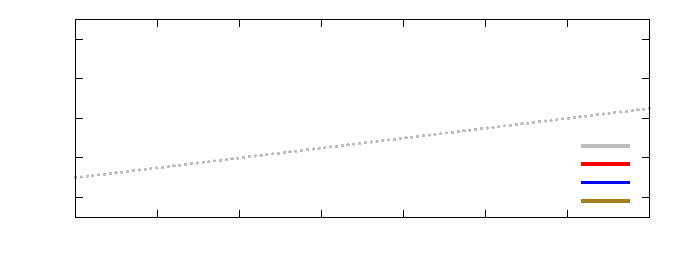
\includegraphics[width={183.00bp},height={169.00bp}]{Quinones}}%
    \gplfronttext
  \end{picture}%
\endgroup
